% ============================================================
% Capítulo: Anexos (Bloque B.17)
% ============================================================
\chapter{Anexos}
\label{cap:anexos}

Este capítulo reúne el material suplementario exigido por la guía
(Bloque~B.17): la cadena de búsqueda bibliográfica ya documentada en el
\autoref{cap:trabajos-relacionados}, el protocolo del instrumento SUS
(aún sin ejecutar), el placeholder del pipeline CI/CD pendiente de
captura manual, el checklist completo de Ralph et~al.\ (2021) verificado
contra \texttt{docs/checklists/ralph2021-engineering-research.md}, y la
matriz de trazabilidad de requisitos parseada desde
\texttt{docs/trazabilidad/matriz.csv} (43 filas de datos + encabezado,
11 columnas, verificadas con un lector CSV antes de transcribirse).

\section{Cadena de búsqueda bibliográfica}
\label{sec:anexo-cadena-busqueda}

La cadena que sigue es la misma documentada en la
\autoref{sec:estrategia-busqueda} del \autoref{cap:trabajos-relacionados}
(``Cadena de búsqueda de referencia'': la usada en las búsquedas
originales del equipo y replicada en la búsqueda dirigida de ese
capítulo). \textbf{No se inventa aquí una cadena nueva}; se traslada
literalmente desde ese archivo fuente.

\begin{quote}
\ttfamily
("library management system" OR "biblioteca" OR "library automation")\\
AND ("QR code" OR RFID OR chatbot OR "recommendation system" OR\\
\phantom{AND (}"generative AI" OR "stored procedure" OR "cache-aside" OR Redis OR ORM)\\
AND (performance OR empirical OR evaluation OR "case study")
\end{quote}

\textbf{Contexto verificado en el mismo capítulo.} Fuentes del acervo:
IEEE~Xplore, ACM~Digital Library, Scopus, ScienceDirect (Elsevier) y
SpringerLink (curación previa), más Crossref e IEEE~Xplore en la
búsqueda dirigida; ventana temporal 2017--2026; criterios de inclusión y
exclusión declarados en la \autoref{sec:estrategia-busqueda}. El flujo de
selección adaptado de PRISMA~2020 aparece en la
\autoref{fig:prisma-flow}.

\section{Protocolo SUS (System Usability Scale)}
\label{sec:anexo-protocolo-sus}

Este anexo documenta únicamente el \textbf{protocolo y el cuestionario}
del instrumento System Usability Scale \citep{brooke1996sus}.
\textbf{No se reportan resultados ni datos de participantes}: al momento
de redactar este documento, $N=0$ de los $N\geq15$ participantes exigidos
por la guía, verificado en la \autoref{sec:res-usabilidad} del
\autoref{cap:resultados} (``Datos crudos. Ninguno todavía.'').

\subsection{Protocolo de aplicación}

\begin{enumerate}[leftmargin=1.2cm]
  \item \textbf{Consentimiento informado.} Antes de la sesión, el
    participante firma la plantilla versionada en
    \texttt{docs/etica/consentimientos/plantilla.md} (los formularios
    firmados \textbf{no} se versionan en el repositorio; ver
    \texttt{docs/etica/ETHICS.md}).
  \item \textbf{Anonimización.} Cada participante recibe un código
    (\texttt{P01}, \texttt{P02}, \ldots); no se registra nombre ni
    correo en los datos de análisis.
  \item \textbf{Muestreo.} Por conveniencia dentro de la comunidad UTEQ
    (roles de dominio lector/bibliotecario), según el protocolo ya
    definido en la \autoref{sec:mm-poblacion}.
  \item \textbf{Tarea previa al cuestionario.} Onboarding de prueba
    descrito en la plantilla de consentimiento (iniciar sesión, crear
    cuenta, editar, dar de baja, cerrar sesión), sin ayuda del equipo
    salvo bloqueo total.
  \item \textbf{Cuestionario.} Tras la tarea, se administran los 10
    ítems de Brooke (1996) en español, con escala Likert de 1 a 5
    (abajo). Duración estimada total de la sesión: 15--20 minutos
    (según la plantilla de consentimiento).
  \item \textbf{Puntuación (cuando existan datos).} La fórmula estándar
    del instrumento produce una puntuación agregada 0--100 por
    participante. \textbf{Aquí no se aplica}: no hay respuestas que
    puntuar.
\end{enumerate}

\subsection{Cuestionario SUS -- 10 ítems originales de Brooke (1996) en español}

Instrucciones al participante: indique su grado de acuerdo con cada
afirmación sobre el sistema que acaba de usar, marcando un solo valor
en la escala de 1 a 5.

\begin{center}
\small
\begin{tabular}{@{}p{0.9\linewidth}@{}}
\toprule
\textbf{Escala Likert (idéntica en los 10 ítems)} \\
\midrule
1 = Totalmente en desacuerdo \quad
2 = En desacuerdo \quad
3 = Neutral \quad
4 = De acuerdo \quad
5 = Totalmente de acuerdo \\
\bottomrule
\end{tabular}
\end{center}

\begin{enumerate}[leftmargin=1.2cm]
  \item Creo que me gustaría utilizar este sistema con frecuencia.
        \hfill (1) (2) (3) (4) (5)
  \item Encontré el sistema innecesariamente complejo.
        \hfill (1) (2) (3) (4) (5)
  \item Pensé que el sistema era fácil de usar.
        \hfill (1) (2) (3) (4) (5)
  \item Creo que necesitaría el apoyo de una persona con conocimientos
        técnicos para poder usar este sistema.
        \hfill (1) (2) (3) (4) (5)
  \item Encontré que las diversas funciones de este sistema estaban
        bien integradas.
        \hfill (1) (2) (3) (4) (5)
  \item Pensé que había demasiada inconsistencia en este sistema.
        \hfill (1) (2) (3) (4) (5)
  \item Imagino que la mayoría de la gente aprendería a utilizar este
        sistema muy rápidamente.
        \hfill (1) (2) (3) (4) (5)
  \item Encontré el sistema muy engorroso de usar.
        \hfill (1) (2) (3) (4) (5)
  \item Me sentí muy confiado/a usando el sistema.
        \hfill (1) (2) (3) (4) (5)
  \item Necesité aprender muchas cosas antes de poder manejarme con
        este sistema.
        \hfill (1) (2) (3) (4) (5)
\end{enumerate}

Los ítems impares son afirmaciones positivas y los pares negativas, según
el diseño original del instrumento \citep{brooke1996sus}. La puntuación
agregada, cuando existan respuestas reales, se calculará con la fórmula
estándar de Brooke; \textbf{no se inventa aquí ninguna puntuación}.

\section{Pipeline CI/CD}
\label{sec:anexo-cicd}

El flujo de integración continua del proyecto está definido en
\texttt{.github/workflows/ci.yml} (job \texttt{build-and-test} sobre
\texttt{ubuntu-latest}, disparado en \texttt{push}/\texttt{pull\_request}
hacia \texttt{main} y \texttt{develop}). La guía pide evidencia visual
de \textbf{tres corridas verdes consecutivas}. Esas capturas
\textbf{aún no están en el repositorio}: el archivo
\texttt{anexos/ci-pipeline-placeholder.png} es un placeholder explícito
para que el equipo las sustituya manualmente cuando existan.

\begin{figure}[h]
\centering
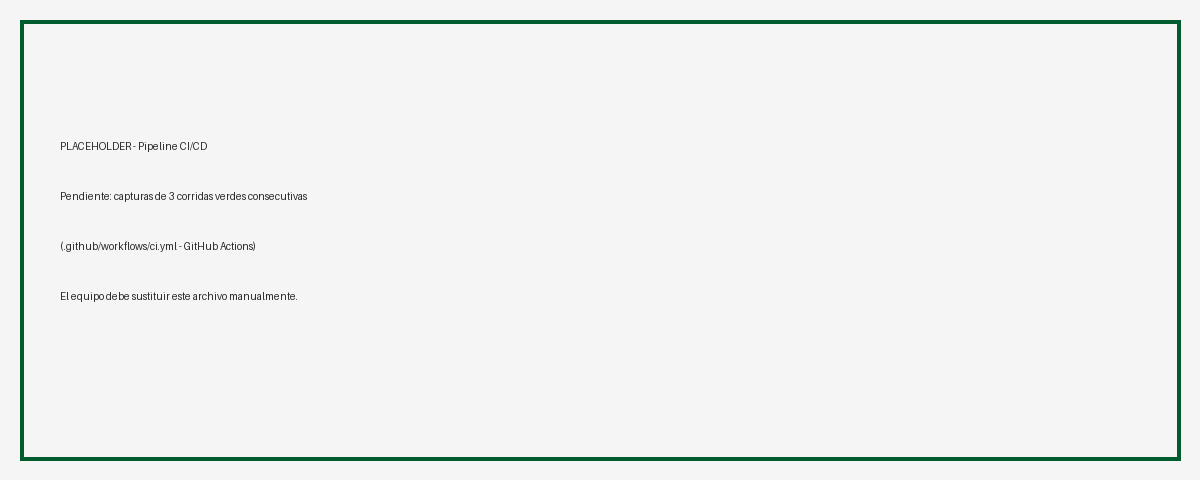
\includegraphics[width=0.95\textwidth]{anexos/ci-pipeline-placeholder.png}
\caption{Placeholder pendiente de captura manual: tres corridas verdes
  consecutivas del pipeline CI/CD de GitHub Actions
  (\texttt{.github/workflows/ci.yml}). Sustituir este archivo por las
  capturas reales cuando estén disponibles; no se fabrican aquí
  capturas ni se declara un estado de CI no verificado en este anexo.}
\label{fig:ci-pipeline-placeholder}
\end{figure}

\section{Checklist Ralph et~al.\ (2021) --- Engineering Research}
\label{sec:anexo-ralph}

El contenido de esta sección es la transcripción tabular del checklist
real versionado en
\texttt{docs/checklists/ralph2021-engineering-research.md}
(fecha 2026-08-13, commit base \texttt{6696bf1}, estándar
``Engineering Research'' de \citet{ralph2021empiricalstandards}).
\textbf{No se resume ni se alteran los veredictos}: se reformatea el
mismo contenido a tablas \texttt{longtable}.

\textbf{Leyenda.} Cumple / Parcial / No cumple / N/A (no aplica al tipo
de artefacto).

\subsection{Atributos esenciales}

\begin{center}
\footnotesize
\renewcommand{\arraystretch}{1.15}
\begin{longtable}{|p{0.7cm}|p{4.2cm}|p{1.6cm}|p{7.0cm}|}
\caption{Checklist Ralph et~al.\ (2021) --- atributos esenciales
  (fuente: \texttt{docs/checklists/ralph2021-engineering-research.md})}
\label{tab:anexo-ralph-esenciales}\\
\hline
\rowcolor{verdeuteq}
\textcolor{white}{\textbf{\#}} &
\textcolor{white}{\textbf{Ítem}} &
\textcolor{white}{\textbf{Estado}} &
\textcolor{white}{\textbf{Evidencia / nota}} \\
\hline
\endfirsthead
\hline
\rowcolor{verdeuteq}
\textcolor{white}{\textbf{\#}} &
\textcolor{white}{\textbf{Ítem}} &
\textcolor{white}{\textbf{Estado}} &
\textcolor{white}{\textbf{Evidencia / nota}} \\
\hline
\endhead
\hline
\endfoot
E1 & Describe el artefacto propuesto con detalle adecuado & \textbf{Cumple} & Modelo C4 completo en Structurizr DSL (\texttt{docs/arquitectura/workspace.dsl}), 13 Architecture Decision Records, y los Capítulos 6 (Diseño y Arquitectura) y 7 (Implementación) del informe describen el flujo completo, los componentes y las decisiones técnicas del sistema. \\
\hline
E2 & Justifica la necesidad, utilidad o relevancia del artefacto propuesto & \textbf{Cumple} & Cap.\ 1 (Introducción), §Contexto y motivación: fricción operativa real y verificable del dominio bibliotecario (registro manual, ausencia de autoservicio). Nota de honestidad ya declarada ahí mismo: el documento evita deliberadamente citar una cifra de ``población afectada'' sin fuente verificada --- la justificación es cualitativa y de dominio, no una cifra inventada. \\
\hline
E3 & Evalúa conceptualmente el artefacto: discute fortalezas, debilidades y limitaciones & \textbf{Cumple} & Cap.\ 12 (Amenazas a la Validez) y Cap.\ 9 (Discusión) discuten debilidades reales (p.\ ej.\ la comparación \texttt{cache\_frío}/\texttt{cache\_caliente} no aísla limpiamente el efecto del caché); los 13 ADR documentan explícitamente los \emph{trade-offs} de cada decisión arquitectónica, no solo la decisión final. \\
\hline
E4 & Evalúa empíricamente el artefacto usando: \emph{action research}, \emph{case study}, experimento controlado, simulación cuantitativa, \emph{benchmarking study}, u otro método con justificación clara & \textbf{Parcial} & El Cap.\ 8 (Resultados) reporta evaluación empírica real (k6, JaCoCo, OWASP, Lighthouse), pero ninguno de sus 5 bloques se declara explícitamente como uno de los 5 métodos canónicos del estándar. El bloque de rendimiento (k6, 5 corridas pareadas \texttt{cache\_frío} vs.\ \texttt{cache\_caliente}) se acerca más a un \emph{benchmarking study}, pero el Cap.\ 5 (Materiales y Métodos) enmarca la metodología con GQM y DSR, no con la taxonomía de Ralph et al. \\
\hline
E5 & Indica claramente cuál de esas metodologías empíricas se usó & \textbf{No cumple} & Consecuencia directa de E4: no existe, en ningún capítulo del informe, una declaración explícita que etiquete la evaluación empírica de SGB-SaaS con la taxonomía de este estándar. Gap real, no solo de redacción. \\
\hline
E6 & O BIEN discute alternativas del estado del arte (con sus fortalezas/debilidades/limitaciones) O BIEN explica por qué no existen O BIEN argumenta de forma convincente que la comparación directa es impráctica & \textbf{Cumple} & Cap.\ 3 (Trabajos Relacionados) completo: 10 trabajos primarios comparados fila a fila (\texttt{tab:trabajos-comparativa}) con columnas explícitas de limitaciones declaradas y pila tecnológica, más una sección dedicada (§Brecha identificada). \\
\hline
E7 & O BIEN compara empíricamente el artefacto con una o más alternativas del estado del arte O BIEN lo compara con \emph{benchmarks} establecidos O BIEN justifica por qué la evaluación comparativa es impráctica & \textbf{Parcial} & La comparación del Cap.\ 3 es descriptiva/cualitativa, no una comparación empírica directa (mismo protocolo de medición aplicado a SGB-SaaS y a un sistema alternativo real). El documento no incluye una frase explícita de tipo ``la comparación empírica directa es impráctica porque ninguno de los sistemas comparables tiene código disponible'' --- la razón es real e inferible de la tabla, pero no está declarada como justificación formal. \\
\hline
E8 & Los supuestos (si los hay) son explícitos, plausibles y no se contradicen entre sí ni con los objetivos de la contribución & \textbf{Cumple} & \texttt{docs/arquitectura/ISO25010.md} declara explícitamente el supuesto de carga (biblioteca universitaria: volumen bajo, ráfagas puntuales); el Cap.\ 5 (§GQM) declara los supuestos del protocolo de medición del caché Redis. \\
\hline
E9 & Usa notación de forma consistente (si se usa alguna notación) & \textbf{N/A} & SGB-SaaS no presenta notación matemática o algorítmica formal (no hay teoremas, pseudocódigo de algoritmos propios ni modelos formales) --- el artefacto es un sistema web, no una contribución analítica. \\
\hline
\end{longtable}
\end{center}

\subsection{Atributos deseables}

\begin{center}
\footnotesize
\renewcommand{\arraystretch}{1.15}
\begin{longtable}{|p{0.7cm}|p{4.2cm}|p{1.6cm}|p{7.0cm}|}
\caption{Checklist Ralph et~al.\ (2021) --- atributos deseables
  (fuente: \texttt{docs/checklists/ralph2021-engineering-research.md})}
\label{tab:anexo-ralph-deseables}\\
\hline
\rowcolor{verdeuteq}
\textcolor{white}{\textbf{\#}} &
\textcolor{white}{\textbf{Ítem}} &
\textcolor{white}{\textbf{Estado}} &
\textcolor{white}{\textbf{Evidencia / nota}} \\
\hline
\endfirsthead
\hline
\rowcolor{verdeuteq}
\textcolor{white}{\textbf{\#}} &
\textcolor{white}{\textbf{Ítem}} &
\textcolor{white}{\textbf{Estado}} &
\textcolor{white}{\textbf{Evidencia / nota}} \\
\hline
\endhead
\hline
\endfoot
D1 & Provee materiales suplementarios: código fuente (si el artefacto es software) y conjuntos de datos de entrada (si aplica) & \textbf{Cumple} & Repositorio completo público bajo MIT (\texttt{docs/capitulos/13-declaraciones.tex}, §13.1); datos crudos de todas las mediciones empíricas versionados en \texttt{docs/mediciones/} (§13.2). \\
\hline
D2 & Justifica, con motivos prácticos o éticos, cualquier elemento faltante del paquete de replicación & \textbf{Cumple} & Los formularios de consentimiento informado firmados de las pruebas SUS se excluyen explícitamente del repositorio por motivos éticos de protección de datos personales, declarado en \texttt{docs/etica/ETHICS.md} y en \texttt{docs/capitulos/13-declaraciones.tex} §13.4. \\
\hline
D3 & Discute la base teórica del artefacto & \textbf{Cumple} & Cap.\ 4 (Marco Teórico) completo: ISO/IEC/IEEE 29148:2018, modelo C4, ISO/IEC 25010, principios REST, JWT, OWASP Top 10, patrones ORM/SP/cache-aside. \\
\hline
D4 & Provee argumentos de corrección para las contribuciones analíticas y teóricas clave (p.\ ej.\ teoremas, análisis de complejidad, demostraciones matemáticas) & \textbf{N/A} & SGB-SaaS no tiene contribuciones analíticas o teóricas de este tipo (no propone un algoritmo nuevo con complejidad demostrable ni un modelo matemático propio). \\
\hline
D5 & Incluye uno o más ejemplos funcionando para ilustrar el artefacto & \textbf{Cumple} & \texttt{docs/postman/coleccion.json} (66 peticiones HTTP reales); listados de código real en el Cap.\ 7 (Implementación). \\
\hline
D6 & Evalúa el artefacto en un contexto relevante para la industria (p.\ ej.\ proyectos de código abierto ampliamente usados, programadores profesionales) & \textbf{No cumple} & SGB-SaaS no tiene todavía un despliegue público ni usuarios reales evaluándolo --- toda la evaluación empírica del Cap.\ 8 se ejecutó en el entorno de desarrollo del propio equipo (\texttt{docker compose}), no en un contexto de uso real. Coincide con $N=0$ en SUS. \\
\hline
\end{longtable}
\end{center}

\subsection{Atributos extraordinarios}

\begin{center}
\footnotesize
\renewcommand{\arraystretch}{1.15}
\begin{longtable}{|p{0.7cm}|p{4.2cm}|p{1.6cm}|p{7.0cm}|}
\caption{Checklist Ralph et~al.\ (2021) --- atributos extraordinarios
  (aspiracionales; no reclamados)}
\label{tab:anexo-ralph-extraordinarios}\\
\hline
\rowcolor{verdeuteq}
\textcolor{white}{\textbf{\#}} &
\textcolor{white}{\textbf{Ítem}} &
\textcolor{white}{\textbf{Estado}} &
\textcolor{white}{\textbf{Nota}} \\
\hline
\endfirsthead
\hline
\rowcolor{verdeuteq}
\textcolor{white}{\textbf{\#}} &
\textcolor{white}{\textbf{Ítem}} &
\textcolor{white}{\textbf{Estado}} &
\textcolor{white}{\textbf{Nota}} \\
\hline
\endhead
\hline
\endfoot
X1 & Contribuye a la comprensión colectiva de prácticas o principios de diseño & \textbf{N/A} & No se reclama --- alcance de PFC académico, no de investigación original en principios de diseño de software. \\
\hline
X2 & Presenta innovaciones revolucionarias con beneficios obvios en el mundo real & \textbf{N/A} & No se reclama, por el mismo motivo. \\
\hline
\end{longtable}
\end{center}

\subsection{Auto-verificación de antipatrones}

Esta subsección corresponde al autoexamen del checklist (no forma parte
del conteo de cumplimiento de los 17 ítems anteriores).

\begin{center}
\footnotesize
\renewcommand{\arraystretch}{1.15}
\begin{longtable}{|p{4.5cm}|p{2.0cm}|p{7.0cm}|}
\caption{Antipatrones del estándar Engineering Research --- autoexamen
  (fuente: \texttt{docs/checklists/ralph2021-engineering-research.md})}
\label{tab:anexo-ralph-antipatrones}\\
\hline
\rowcolor{verdeuteq}
\textcolor{white}{\textbf{Antipatrón}} &
\textcolor{white}{\textbf{¿Se evitó?}} &
\textcolor{white}{\textbf{Nota}} \\
\hline
\endfirsthead
\hline
\rowcolor{verdeuteq}
\textcolor{white}{\textbf{Antipatrón}} &
\textcolor{white}{\textbf{¿Se evitó?}} &
\textcolor{white}{\textbf{Nota}} \\
\hline
\endhead
\hline
\endfoot
Sobreestimar la novedad de la contribución & \textbf{Evitado} & Cap.\ 3, §Brecha identificada, declara dos advertencias explícitas de honestidad metodológica que acotan la afirmación de brecha. \\
\hline
Omitir detalles conceptuales clave centrándose solo en aspectos incidentales de implementación & \textbf{Evitado} & Cap.\ 4 (Marco Teórico) y Cap.\ 6 (Diseño) cubren extensamente el ``por qué'' antes que el ``cómo''. \\
\hline
La evaluación consiste únicamente en recoger opiniones de usuarios & \textbf{Evitado} & $N=0$ en SUS --- no hay ninguna opinión de usuario recogida todavía; el resto de la evaluación (k6, JaCoCo, OWASP, Lighthouse) es técnica. \\
\hline
La evaluación consiste únicamente en datos de rendimiento cuantitativos no comparados contra \emph{benchmarks} o alternativas establecidas & \textbf{Riesgo parcial} & El bloque de rendimiento (k6) compara dos escenarios internos del propio SGB-SaaS, no contra un sistema alternativo externo ni contra un \emph{benchmark} de la industria --- coincide con el gap de E7. \\
\hline
Diseño no experimental (un solo grupo, sin repetición) & \textbf{Riesgo parcial} & El bloque de rendimiento sí es repetido (5 corridas, Wilcoxon). El bloque de Lighthouse, con solo $n=2$ corridas (ambas móvil), es más cercano al antipatrón. \\
\hline
Evaluación usando ejemplos de juguete (a veces presentados como ``estudios de caso'') & \textbf{Evitado} & Los datos de ejemplo son libros reales con ISBN real (\texttt{db/seed.sql}); los escenarios de carga de k6 reflejan el perfil de uso declarado de una biblioteca universitaria. \\
\hline
\end{longtable}
\end{center}

\subsection{Resumen de cumplimiento (verificado)}

Conteo recalculado al transcribir las 17 filas del checklist fuente
(9 esenciales + 6 deseables + 2 extraordinarios):

\begin{table}[h]
\centering
\small
\begin{tabular}{lcccc}
\toprule
Categoría & Cumple & Parcial & No cumple & N/A \\
\midrule
Esenciales (9 ítems) & 5 & 2 & 1 & 1 \\
Deseables (6 ítems) & 4 & 0 & 1 & 1 \\
Extraordinarios (2 ítems) & 0 & 0 & 0 & 2 \\
\midrule
\textbf{Total (17 ítems)} & \textbf{9} & \textbf{2} & \textbf{2} & \textbf{4} \\
\bottomrule
\end{tabular}
\caption{Resumen de cumplimiento Ralph et~al.\ (2021), idéntico al del
  archivo fuente \texttt{docs/checklists/ralph2021-engineering-research.md}}
\label{tab:anexo-ralph-resumen}
\end{table}

\section{Matriz de trazabilidad}
\label{sec:anexo-matriz}

La tabla siguiente transcribe \textbf{las 43 filas de datos} de
\texttt{docs/trazabilidad/matriz.csv}, leídas con el módulo
\texttt{csv} de Python (no copia visual). Verificación previa a la
transcripción: 1 fila de encabezado + 43 filas de datos = 44 filas
totales; 11 columnas en todas las filas
(\texttt{id\_requisito}, \texttt{tipo}, \texttt{prioridad\_moscow},
\texttt{historia\_usuario}, \texttt{caso\_de\_uso},
\texttt{modulo\_codigo}, \texttt{endpoint\_api},
\texttt{prueba\_automatizada}, \texttt{tipo\_acceso},
\texttt{evidencia\_empirica}, \texttt{estado}). Las celdas con rayas
largas (``---'') en el CSV se conservan como tales.

\begin{landscape}
\begin{center}
\scriptsize
\renewcommand{\arraystretch}{1.05}
\setlength{\tabcolsep}{2pt}
\begin{longtable}{|p{1.35cm}|p{1.1cm}|p{1.1cm}|p{2.0cm}|p{1.7cm}|p{2.3cm}|p{2.4cm}|p{3.0cm}|p{2.0cm}|p{2.6cm}|p{1.3cm}|}
\caption{Matriz de trazabilidad de requisitos (43 filas; fuente:
  \texttt{docs/trazabilidad/matriz.csv})}
\label{tab:anexo-matriz}\\
\hline
\rowcolor{verdeuteq}
\textcolor{white}{\textbf{ID}} &
\textcolor{white}{\textbf{Tipo}} &
\textcolor{white}{\textbf{MoSCoW}} &
\textcolor{white}{\textbf{HU}} &
\textcolor{white}{\textbf{CU}} &
\textcolor{white}{\textbf{Módulo}} &
\textcolor{white}{\textbf{Endpoint}} &
\textcolor{white}{\textbf{Prueba}} &
\textcolor{white}{\textbf{Acceso}} &
\textcolor{white}{\textbf{Evidencia}} &
\textcolor{white}{\textbf{Estado}} \\
\hline
\endfirsthead
\hline
\rowcolor{verdeuteq}
\textcolor{white}{\textbf{ID}} &
\textcolor{white}{\textbf{Tipo}} &
\textcolor{white}{\textbf{MoSCoW}} &
\textcolor{white}{\textbf{HU}} &
\textcolor{white}{\textbf{CU}} &
\textcolor{white}{\textbf{Módulo}} &
\textcolor{white}{\textbf{Endpoint}} &
\textcolor{white}{\textbf{Prueba}} &
\textcolor{white}{\textbf{Acceso}} &
\textcolor{white}{\textbf{Evidencia}} &
\textcolor{white}{\textbf{Estado}} \\
\hline
\endhead
\hline
\endfoot
REQ-F-001 & funcional & Must & HU-AUTH-01 & CU-AUTH-01 & AuthController/AuthService & POST /api/auth/registro & AuthServiceTest.registroCorreoDuplicado (criterio 2, correo duplicado); AuthServiceTest.registroExitoso\_dejaAlUsuarioPendienteDeVerificacionYEnviaElCodigo + AuthControllerTest.registro\_datosValidos\_devuelve201ConUsuarioCreado (criterio 1, flujo exitoso --- 201 y estado, cada uno cubre una mitad ya que el controller test mockea AuthService); AuthControllerTest.registro\_passwordCorta\_devuelve400ProblemDetail (criterio 3, contraseña corta, aislado --- nuevo) & CRUD-ORM & --- & verificado \\
\hline
REQ-F-002 & funcional & Must & HU-AUTH-02 & CU-AUTH-02 & AuthController/AuthService & POST /api/auth/login & AuthServiceTest.login* (5 tests) & CRUD-ORM & docs/mediciones/sec/2026-07-30-owasp-a07-fix-rate-limiting-login.md; docs/mediciones/sec/2026-07-30-owasp-a09-fix-logging-autenticacion.md & verificado \\
\hline
REQ-F-003 & funcional & Must & HU-AUTH-03 & CU-AUTH-03 & AuthController/AuthService & POST /api/auth/logout & AuthServiceTest.logoutGuardaTokenEnBlacklist & CRUD-ORM (bitácora) + Redis (blacklist) & docs/mediciones/sec/2026-07-30-owasp-a09-fix-logging-autenticacion.md & verificado \\
\hline
REQ-F-004 & funcional & Must & HU-AUTH-04 & CU-AUTH-04 & AuthController/AuthService & POST /api/auth/refresh & AuthServiceTest.refreshConTokenValido & CRUD-ORM & docs/mediciones/sec/2026-07-21-cookie-refresh-token.md & verificado \\
\hline
REQ-F-005 & funcional & Must & HU-LIB-01 & CU-LIB-01 & LibroController/LibroService & GET /api/v1/libros; GET /api/v1/libros/\{id\} & LibroServiceTest.listar\_retornaPaginaDeLibros; .buscarPorId\_cuandoNoExiste\_lanzaEntityNotFound; LibroControllerSecurityTest (4 tests, @PreAuthorize real via MockMvc) & CRUD-ORM & docs/mediciones/sec/2026-07-30-owasp-a01-fix-rol-admin-libros.md & verificado \\
\hline
REQ-F-006 & funcional & Must & HU-LIB-02 & CU-LIB-02 & LibroController/LibroService & POST /api/v1/libros; PUT /api/v1/libros/\{id\}; DELETE /api/v1/libros/\{id\} & LibroServiceTest.crearLibro\_cuandoIsbnNuevo\_retornaDTO; .crearLibro\_cuandoIsbnDuplicado\_lanzaExcepcion; .eliminar\_cuandoExiste\_loMarcaDadoDeBaja; LibroControllerSecurityTest (4 tests, @PreAuthorize real via MockMvc) & CRUD-ORM & docs/mediciones/sec/2026-07-30-owasp-a01-fix-rol-admin-libros.md & verificado \\
\hline
REQ-F-007 & funcional & Must & HU-01 (Cajas) & CU-01 (Cajas) & PrestamoController/PrestamoService & POST /api/v1/prestamos & PrestamoServiceTest.crear\_conDatosValidos\_invocaProcedimientoYRetornaDTO; PrestamoMultaProcedureIntegrationTest (6 tests, integracion real contra Postgres) & SP (sp\_crear\_prestamo) & docs/mediciones/backend/2026-07-29-flujo-prestamo-devolucion-multa-e2e.md & verificado \\
\hline
REQ-F-008 & funcional & Must & HU-02 (Cajas) & CU-02 (Cajas) & PrestamoController/PrestamoService & POST /api/v1/prestamos/\{id\}/devolucion & PrestamoServiceTest.registrarDevolucion\_sinAtraso\_noGeneraMulta; .registrarDevolucion\_conAtraso\_generaMulta; PrestamoMultaProcedureIntegrationTest.registrarDevolucion\_* (3 tests) & SP (sp\_registrar\_devolucion) & docs/mediciones/backend/2026-07-29-flujo-prestamo-devolucion-multa-e2e.md & verificado \\
\hline
REQ-F-009 & funcional & Must & HU-F02 (Panama) & CU-F02 (Panama) & PrestamoController/PrestamoService + PrestamosLectorComponent & GET /api/v1/prestamos/usuario/\{id\}; GET /api/v1/prestamos/usuario/\{id\}/activos & PrestamoServiceTest.listarPorUsuario\_cuandoLectorPideOtroUsuario\_lanzaAccesoDenegado; prestamos-lector.component.spec.ts (2 tests) & CRUD-ORM & docs/mediciones/frontend/2026-07-30-flujo-frontend-prestamos-reservaciones-multas-e2e.md & verificado \\
\hline
REQ-F-010 & funcional & Should & --- & --- & PrestamoController/PrestamoService & GET /api/v1/prestamos/reportes/libros-mas-prestados & PrestamoServiceTest.reporteLibrosMasPrestados\_sinLimite\_aplicaDefaultDiez & SP (fn\_reporte\_libros\_mas\_prestados) & --- & implementado \\
\hline
REQ-F-011 & funcional & Must & HU-03 (Cajas); HU-F03 (Panama) & CU-03 (Cajas); CU-F03 (Panama) & ReservacionController/ReservacionService + ReservacionesComponent & POST /api/v1/reservaciones & ReservacionServiceTest.crear\_* (4 tests); reservaciones.component.spec.ts (2 tests) & CRUD-ORM & docs/mediciones/frontend/2026-07-30-flujo-frontend-prestamos-reservaciones-multas-e2e.md & verificado \\
\hline
REQ-F-012 & funcional & Must & HU-F03 (Panama, inferida --- el mismo componente cubre creación y listado, no hay HU dedicada solo a listar) & CU-F03 (Panama) & ReservacionController/ReservacionService & GET /api/v1/reservaciones/usuario/\{id\} & ReservacionServiceTest.listarPorUsuario\_cuandoLectorPideOtroUsuario\_lanzaAccesoDenegado & CRUD-ORM & docs/mediciones/frontend/2026-07-30-flujo-frontend-prestamos-reservaciones-multas-e2e.md & verificado \\
\hline
REQ-F-013 & funcional & Must & HU-F01 (Panama) & CU-F01 (Panama) & MultaController/MultaService + MultasComponent & GET /api/v1/multas/usuario/\{id\} & MultaServiceTest.listarPorUsuario\_cuandoLectorPideOtroUsuario\_lanzaAccesoDenegado; multas.component.spec.ts (2 tests) & CRUD-ORM & docs/mediciones/frontend/2026-07-30-flujo-frontend-prestamos-reservaciones-multas-e2e.md & verificado \\
\hline
REQ-F-014 & funcional & Must & HU-04 (Cajas) & CU-04 (Cajas) & MultaController/MultaService & POST /api/v1/multas/\{id\}/pago & MultaServiceTest.pagar\_invocaProcedimientoYRetornaDTO; .pagar\_conOtrasMultasPendientes\_noDesbloqueaUsuario; PrestamoMultaProcedureIntegrationTest.pagarMulta\_unicaPendiente\_desbloqueaUsuario & SP (sp\_pagar\_multa) & docs/mediciones/backend/2026-07-29-flujo-prestamo-devolucion-multa-e2e.md & verificado \\
\hline
REQ-F-015 & funcional & Must & HU-05 (Cajas) & CU-05 (Cajas) & MultaController/MultaService & POST /api/v1/multas/\{id\}/anulacion & MultaServiceTest.anular\_conRolGerente\_resuelveRolDesdeAuthentication; .anular\_conRolAdmin\_resuelveRolAdmin; .anular\_sinRolGerenteOAdmin\_lanzaAccesoDenegado; PrestamoMultaProcedureIntegrationTest.anularMulta\_* (2 tests) & SP (sp\_anular\_multa) & docs/mediciones/backend/2026-07-29-flujo-prestamo-devolucion-multa-e2e.md & verificado \\
\hline
REQ-F-016 & funcional & Must & HU-F04 (Panama) & CU-F04 (Panama) & PrestamosGestionComponent (frontend) & POST /api/v1/prestamos; POST /api/v1/prestamos/\{id\}/devolucion (mismos endpoints que REQ-F-007/REQ-F-008, capa UI) & prestamos-gestion.component.spec.ts (2 tests) & N/A (capa UI, sin acceso directo a BD) & docs/mediciones/frontend/2026-07-30-flujo-frontend-prestamos-reservaciones-multas-e2e.md & verificado \\
\hline
REQ-NF-001 & no funcional & Must & HU-AUTH-03 & CU-AUTH-03 & AuthService/JwtService (ADR-003) & POST /api/auth/logout & AuthServiceTest.logoutGuardaTokenEnBlacklist & N/A (Redis, no BD) & docs/mediciones/sec/2026-07-30-owasp-a09-fix-logging-autenticacion.md & verificado \\
\hline
REQ-NF-002 & no funcional & Must & HU-AUTH-04 & CU-AUTH-04 & AuthController/AuthService (adr-012-cookies-jwt.md) & POST /api/auth/login; POST /api/auth/refresh; POST /api/auth/logout & AuthServiceTest.refreshConTokenValido & CRUD-ORM & docs/mediciones/sec/2026-07-21-cookie-refresh-token.md & verificado \\
\hline
REQ-NF-003 & no funcional & Should & --- (requisito a nivel de configuración, ver CU-LIB-01) & CU-LIB-01 & LibroService (adr-008-ttl-cache-libros.md) & GET /api/v1/libros & --- & CRUD-ORM (dato subyacente) + cache Redis (TTL configurable) & docs/mediciones/sec/2026-07-21-cache-libros-ttl.md & implementado \\
\hline
REQ-NF-004 & no funcional & Must & HU-01 (Cajas, lado SP); HU-AUTH-06 (Marlon, lado ORM) & CU-01 (Cajas); CU-AUTH-06 (Marlon) & transversal: PrestamoService/MultaService/ReservacionService (SP) + AuthService (ORM) (adr-006-acceso-datos-orm-sp.md) & N/A (decisión de arquitectura transversal) & PrestamoMultaProcedureIntegrationTest (6 tests, SP real); AuthServiceTest (8 tests, ORM) & Híbrido: SP (préstamos/multas/reservaciones complejas) + CRUD-ORM (auth/libros/bitácora, CRUD de una sola tabla) & docs/mediciones/backend/2026-07-29-flujo-prestamo-devolucion-multa-e2e.md & verificado \\
\hline
REQ-NF-005 & no funcional & Should & N/A - decisión arquitectónica & N/A - decisión arquitectónica & db/schema.sql + db/seed.sql + Flyway (adr-013-estrategia-schema-reproducible.md) & N/A & --- & N/A (esquema/infraestructura, no aplica CRUD-ORM/SP) & --- & implementado \\
\hline
REQ-NF-006 & no funcional & Must & HU-AUTH-05 & CU-AUTH-05 & LoginRateLimiter & POST /api/auth/login & LoginRateLimiterTest (6 tests); AuthServiceTest.login*RateLimit* (3 tests) & N/A (Redis, no BD) & docs/mediciones/sec/2026-07-30-owasp-a07-fix-rate-limiting-login.md & verificado \\
\hline
REQ-NF-007 & no funcional & Must & HU-AUTH-06 & CU-AUTH-06 & AuthService/BitacoraAuditoriaRepository & POST /api/auth/login; POST /api/auth/logout & AuthServiceTest.loginExitosoReseteaContadorDeRateLimit; .loginFallidoIncrementaContadorDeRateLimit; .logoutGuardaTokenEnBlacklist (verifican bitacoraAuditoriaRepository.save()) & CRUD-ORM & docs/mediciones/sec/2026-07-30-owasp-a09-fix-logging-autenticacion.md & verificado \\
\hline
REQ-NF-008 & no funcional & Should & N/A - decisión arquitectónica & N/A - decisión arquitectónica & toda la capa de persistencia (adr-011-gestor-base-datos.md) & N/A & PrestamoMultaProcedureIntegrationTest (corre contra Postgres real, no contra un mock) & N/A (elección de motor de base de datos) & --- & implementado \\
\hline
REQ-NF-009 & no funcional & Should & N/A - decisión arquitectónica & N/A - decisión arquitectónica & docker-compose.yml + Dockerfiles (adr-007-estrategia-despliegue.md) & N/A & --- & N/A & --- & implementado \\
\hline
REQ-NF-010 & no funcional & Must & HU-AUTH-07 & CU-AUTH-07 & Spring Security (@PreAuthorize) + SPs (defensa en profundidad) (adr-010-autenticacion-jwt-rbac.md) & transversal (todos los endpoints con @PreAuthorize) & MultaServiceTest.anular\_sinRolGerenteOAdmin\_lanzaAccesoDenegado; .listarPorUsuario\_cuandoLectorPideOtroUsuario\_lanzaAccesoDenegado (+ patrones equivalentes en Prestamo/ReservacionServiceTest) & N/A (control de acceso, no patrón de acceso a datos) & docs/mediciones/sec/2026-07-30-owasp-a01-control-acceso-roto.md & verificado \\
\hline
REQ-NF-011 & no funcional & Must & HU-AUTH-07 & CU-AUTH-07 & transversal (@PreAuthorize + AuthorizationDeniedException handler) & transversal & MultaServiceTest.anular\_sinRolGerenteOAdmin\_lanzaAccesoDenegado & N/A & docs/mediciones/sec/2026-07-30-owasp-a01-control-acceso-roto.md & verificado \\
\hline
REQ-NF-012 & no funcional & Should & N/A - decisión arquitectónica & N/A - decisión arquitectónica & SecurityConfig.java (forward-headers-strategy) / adr-015-tls-transporte.md & N/A & --- & N/A (decisión de arquitectura + preparación de backend, no aplica CRUD-ORM/SP) & docs/mediciones/sec/2026-07-30-owasp-a02-fallo-criptografico.md; docs/mediciones/sec/2026-08-10-owasp-a02-fix-tls-transporte.md (decisión ADR-015 y forward-headers-strategy cerrados; verificación de despliegue real completada: header \texttt{Strict-Transport-Security} confirmado activo en producción por \texttt{curl}, 18-ago-2026 -- A02 cerrado en su totalidad) & implementado \\
\hline
REQ-NF-013 & no funcional & Must & HU-01 (Cajas); HU-LIB-02 (Marlon) & CU-01 (Cajas); CU-LIB-02 (Marlon) & transversal (JPA parametrizado + SPs con parámetros tipados) & transversal & AuthServiceTest.registroConPayloadDeInyeccionSql\_seGuardaComoTextoLiteralSinLanzarExcepcion (nuevo, replica como regresión permanente el caso 2 de la auditoría manual) & Híbrido: SP + CRUD-ORM (ambos parametrizados, sin concatenación de SQL) & docs/mediciones/sec/2026-07-30-owasp-a03-inyeccion.md & verificado \\
\hline
REQ-NF-014 & no funcional & Should & N/A - decisión arquitectónica & N/A - decisión arquitectónica & SecurityConfig.java (CSP) / application.yml (perfil prod) / Dockerfile backend / frontend-angular/nginx.conf & N/A & --- & N/A (configuración de seguridad transversal, no aplica CRUD-ORM/SP) & docs/mediciones/sec/2026-07-30-owasp-a05-mala-configuracion-seguridad.md; docs/mediciones/sec/2026-08-10-owasp-a05-fix-csp-stacktrace-swagger-nonroot.md (backend: CSP, stacktraces, Swagger en prod y usuario no-root cerrados; CSP de nginx.conf en frontend queda fuera de alcance de esta rama) & implementado \\
\hline
REQ-NF-015 & no funcional & Should & N/A - decisión arquitectónica & N/A - decisión arquitectónica & .github/workflows/ci.yml + Makefile + config/OpenApiConfig.java (Módulo 13/14/11.1) & N/A & --- & N/A (infraestructura de CI/documentación, no aplica CRUD-ORM/SP) & --- & implementado \\
\hline
REQ-F-017 & funcional & Should & HU-CFG-01 & CU-CFG-01 & ConfiguracionSistemaController/ConfiguracionSistemaService & GET /api/v1/configuracion; PUT /api/v1/configuracion/\{clave\} & ConfiguracionSistemaServiceTest (6 tests); ConfiguracionSistemaControllerSecurityTest (4 tests) & CRUD-ORM + cache en memoria & --- & implementado \\
\hline
REQ-F-018 & funcional & Should & HU-PRE-03 & CU-07 & PrestamoController/PrestamoService (renovar) & POST /api/v1/prestamos/\{id\}/renovacion & PrestamoServiceTest (6 tests nuevos: 50-55) & CRUD-ORM (validación en Java, sin SP nuevo) & --- & implementado \\
\hline
REQ-F-019 & funcional & Should & HU-PRE-04 & CU-01 & PrestamoService (crear, resolverUsuarioId)/CredencialQrController/CredencialQrService & GET /api/v1/credencial-qr/mi-credencial; POST /api/v1/prestamos (con credencialQrToken) & CredencialQrServiceTest (5 tests); PrestamoServiceTest (4 tests nuevos: 12-15) & CRUD-ORM + generacion de imagen (ZXing) & --- & implementado \\
\hline
REQ-F-020 & funcional & Should & --- & --- & AuthController/AuthService/VerificacionCorreoService & POST /api/auth/verificar-correo & AuthServiceTest.registroExitoso\_dejaAlUsuarioPendienteDeVerificacionYEnviaElCodigo; .verificarCorreo\_* (2 tests nuevos); VerificacionCorreoServiceTest (5 tests) & Redis (código OTP con TTL, sin tabla nueva) + SMTP (EmailService) & --- & implementado \\
\hline
REQ-F-021 & funcional & Should & --- & --- & NotificacionController/NotificacionService & GET /api/v1/notificaciones/usuario/\{id\} & NotificacionServiceTest (6 tests); NotificacionControllerSecurityTest (4 tests) & CRUD-ORM & --- & implementado \\
\hline
REQ-F-022 & funcional & Should & --- & --- & NotificacionVencimientoScheduler/NotificacionService/PrestamoService (registrarDevolucion)/ReservacionScheduler & N/A (job periódico + wiring interno de alertas de vencimiento/multa/reserva caducada; sin endpoint propio) & NotificacionVencimientoSchedulerTest (3 tests); PrestamoServiceTest.registrarDevolucion\_* (2 tests); NotificacionServiceTest.generarAlertaVencimiento\_*/notificarMulta\_*/notificarReservaCaducada\_* (4 tests); EmailServiceTest (2 tests) & CRUD-ORM + SMTP & --- & implementado \\
\hline
REQ-F-023 & funcional & Should & HU-ADM-01 & CU-ADM-01 & UsuarioAdminController/UsuarioAdminService & GET /api/v1/admin/usuarios; PATCH /api/v1/admin/usuarios/\{id\}/rol; PATCH /api/v1/admin/usuarios/\{id\}/estado & UsuarioAdminServiceTest (9 tests); UsuarioAdminControllerSecurityTest (8 tests) & CRUD-ORM (bitácora) & --- & implementado \\
\hline
REQ-F-024 & funcional & Should & HU-AUD-01 & CU-AUD-01 & AuditoriaController/AuditoriaService & GET /api/v1/auditoria & AuditoriaServiceTest (4 tests); AuditoriaControllerSecurityTest (5 tests) & CRUD-ORM & --- & implementado \\
\hline
REQ-F-025 & funcional & Should & --- & --- & PrestamoController/PrestamoService & GET /api/v1/prestamos/reportes/morosidad & PrestamoServiceTest.reporteMorosidad\_sinLimite\_aplicaDefaultDiez; .reporteMorosidad\_conFilas\_mapeaProjectionADTO & SP (fn\_reporte\_indice\_morosidad) & --- & implementado \\
\hline
REQ-F-026 & funcional & Should & --- & --- & PrestamoController/PrestamoService & GET /api/v1/prestamos/reportes/uso & PrestamoServiceTest.reporteUsoPorPeriodo\_conGranularidadValida\_invocaRepositorioConValorNormalizado; .reporteUsoPorPeriodo\_conGranularidadInvalida\_lanzaExcepcion & SP (fn\_reporte\_uso\_por\_periodo) & --- & implementado \\
\hline
REQ-F-027 & funcional & Should & --- & --- & PrestamoController/ReportePdfService & GET /api/v1/prestamos/reportes/morosidad/pdf & ReportePdfServiceTest.generarReporteMorosidad\_conFilas\_generaPdfConDatosEsperados; .generarReporteMorosidad\_sinFilas\_generaPdfConMensajeVacio & SP (fn\_reporte\_indice\_morosidad) + PDF en memoria (iText) & --- & implementado \\
\hline
REQ-F-028 & funcional & Should & --- & --- & ChatbotController/ChatbotService (adr-016-gemini-privacidad.md) & POST /api/v1/chatbot/mensajes; GET /api/v1/chatbot/sesiones/\{id\}/historial & ChatbotServiceTest (8 tests); ChatbotControllerSecurityTest (5 tests); ChatbotRateLimiterTest (5 tests); ChatbotServiceIntegrationTest (@Disabled, manual con GEMINI\_API\_KEY real) & CRUD-ORM + Redis (rate limit) + API externa (Gemini, HTTP directo) & --- & implementado \\
\hline
\end{longtable}
\end{center}
\end{landscape}
